\section{Introduction}
\label{chapter:intro}
When developing a web application, there are numerous issues the application writer must consider. One of the most used languages when designing the front-end of a web application is JavaScript\cite{javascript_popularity}, a dynamically typed, multi-paradigm programming language.\cite{javascript_info} Unfortunately, JavaScript suffers from a couple of drawbacks and attacks towards the language through Cross-Site Scripting (XSS) were on the third place on the OWASP Top 10 in 2013.\cite{owasp_xss_rank} In a XSS attack, the attacker manages to inject JavaScript code into websites that are considered secure.\cite{owasp_xss, excess_xss} These injections can do anything from harmless pranks (e.g. showing an alert box) to redirecting the non-suspecting user to a fake website to steal valuable information. When an attack like XSS succeeds, the culprit is usually non-escaped input from the users. If a website directly includes the user input, an attacker can insert input that will be treated as code by the victim.\cite{excess_xss} Examples of valuable information retained by the browser for an attacker are cookies and session tokens.
\subsection{Problems with JavaScript}
JavaScript suffers from two big problems, namely
\begin{itemize}
  \item It is weak, dynamically typed.
  \item It can gain access to sensitive information from the browser.
\end{itemize}
\subsubsection{Weak dynamic typing}
There are several odd features one can use in JavaScript due to the weak dynamic typing. Where a statically typed language (e.g. Java) would give a compile error, the JavaScript code will be run and perhaps succeed but with unexpected results. Figure \ref{fig:error_java} shows a logical error that is caught at compile time in Java. If the code in Figure \ref{fig:error_java} would be allowed to run, it would be up to the runtime environment to determine how the code would be interpreted. The same error in JavaScript i shown in Figure \ref{fig:error_js}. Since JavaScript does not have any static type checking the decision on how to interpret the code will be made at runtime. Instead of failing and raising a runtime error, JavaScript will convert the \textbf{true} value into a number which in this case corresponds to the number \textbf{1}. Hence the addition will be evaluated to \textbf{3}. Situatuations like that, where a clear type error is allowed to propagate and potentially change the state of the application should be considered dangerous and prone to producing bugs.

Another issue with the weak type system in JavaScript can be seen in Figure \ref{fig:js_comparison}. It is perfectly legal to compare a function with an array in JavaScript. The code in Figure \ref{fig:js_comparison} will evaluate to \textbf{true}. This can in turn make it very difficult to find potential bugs since JavaScript will try and convert values of different types to the same types and then make the comparison. In e.g. Java, the comparison in Figure \ref{fig:js_comparison} would not go through the type checker.
\begin{figure}[h]
  \lstset{language=Java}
  \begin{lstlisting}
    int a = 2;
    boolean b = true;
    a + b;  // This should not be allowed to be run
  \end{lstlisting}
  \caption{Logical error in Java}
  \label{fig:error_java}
\end{figure}
\begin{figure}[h]
  \begin{lstlisting}
    var a = 2;
    var b = true;
    a + b;  // This will evaluate to 3
  \end{lstlisting}
  \caption{Logical error in JavaScript}
  \label{fig:error_js}
\end{figure}
\begin{figure}[h]
  \begin{lstlisting}
    (function(x) { return x * x; }) > [1,2,3];
  \end{lstlisting}
  \caption{Weird comparison in JavaScript}
  \label{fig:js_comparison}
\end{figure}

\subsubsection{Sensitive information in the browser}
The browser has access to several different types of sensitive information and can be used by an attacker to get the sensitive information. JavaScript can gain access to e.g. cookies, send HTTP requests and make arbitrary DOM modifications. If untrusted JavaScript is executed in a victims browser, the attacker can, among other things, perform the following attacks:
\begin{itemize}
  \item \textbf{Cookie theft}, where the attacker can gain access to the victim's cookies that are associated with the current website.
  \item \textbf{Keylogging}, where the attacker can create and register a keyboard event listener and send the keystrokes to the attacker's own server in order to potentially record passwords, credit card information etc.
  \item \textbf{Phishing}, where the attacker can insert fake forms by manipulating the DOM and fool the user to submit sensitive information which will be redirected to the attacker.
\end{itemize}
\subsubsection{Examples of attempts to solutions}
There have been several attempts of providing a more secure type system to JavaScript, everything from creating a statically typed language that compiles to JavaScript to a compiler from an already existing programming language and compile it to JavaScript to a static type checker. Examples of attempted soultions are
\begin{itemize}
  \item \textbf{TypeScript}\cite{typescript}, a typed superset of JavaScript that compiles to plain JavaScript.
  \item \textbf{TeJaS}\cite{tejas-art,tejas-git}, which allows you to annotate type signatures as comments in the JavaScript code and then type checks the code.
  \item \textbf{GHCJS}\cite{ghcjs} and \textbf{Haste}\cite{haste-lang,haste-symposium}, which compiles from Haskell, a statically typed, high-level functional programming language\cite{haskell}, to JavaScript.
\end{itemize}

When looking at the other major flaw, namely that JavaScript has access to sensitive information that is stored within the browser, the current solution as of now is to sandbox the script and run it in a secure environment. There are mainly three ways of doing this.
\begin{itemize}
  \item Wrap the script inside a call to with and pass a faked window object and execute the code with eval.
  \item Use an iframe and set the sandbox attribute to either not allow scripts to run or have it be run within that iframe only. Unfortunately, as explained in \cite{js_in_js}, iframes have some issues as well.
  \item Use existing tools to help sandbox third party code, such as:
    \begin{itemize}
      \item \textbf{JavaScript in JavaScript}\cite{js_in_js}, an interpreter that allows an application to execute third-party scripts in a completely isolated, sandboxed environment.
      \item \textbf{Caja}\cite{caja_spec}, a compiler to make third party code safe to embed within a website.
    \end{itemize}
\end{itemize}

\subsection{Information-Flow Control}
Confidentiality in any system is important. Unfortunately, there are few built in mechanisms for ensuring end-to-end confidentiality policies.\cite{ifc-jsac} The general idea behind information flow control is to tag the data with one of two security levels, \emph{high} or \emph{low}. These levels can be seen as either private data (high security level) or public data (low security level). Figure \ref{fig:normal_flow} explains the flow in an application developed with the core language of JavaScript. In JavaScript, there is no way of controlling the flow by dividing the different values of the application into either a high or low context. It is more of a straight line from the input to the output. However, if an implementation of a system that enforces information-flow control were in place, the flow could be seen as in Figure \ref{fig:controlled_flow}. The only flow that is not allowed is a flow from a high context to a low context. All the other flows, i.e. low to low, low to high and high to high, are valid. A system that enforces information-flow control will help in ensuring end-to-end confidentiality.
\begin{figure}[h]
  \begin{subfigure}{.5\textwidth}
    \includegraphics[scale=0.65]{images/flow_normal.eps}
    \caption{Normal information flow}
    \label{fig:normal_flow}
  \end{subfigure}
  \begin{subfigure}{.5\textwidth}
    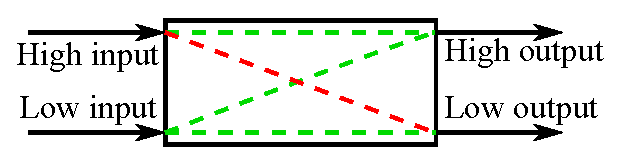
\includegraphics[scale=0.65]{images/flow_controlled.eps}
    \caption{Controlled information flow}
    \label{fig:controlled_flow}
  \end{subfigure}
  \caption{Different kinds of flow in a web application}
  \label{fig:flows}
\end{figure}
